\documentclass[12pt]{cls}
%set MUN Thesis Guidelines margins
\usepackage[left=3.8cm, right=2.5cm, top=3cm, bottom=3cm]{geometry}

%lists package and bullet formats
\usepackage{paralist}
\usepackage{bbding}
%enhanced graphics support
\usepackage{graphicx}
%formatting for websites and e-mail addresses
\usepackage{url}
%pageheaders and footers in LaTeX2e
\usepackage{fancyhdr}
%footnote options
\usepackage{footmisc}
%algorithms
\usepackage{algorithmic}
%source code printer
\usepackage{listings}
%read/write verbatim TeX code
\usepackage{fancyvrb}

\setlength{\parskip}{16pt plus 1pt minus 1pt}



%THIS IS WHERE YOU ENTER THE TITLE OF YOUR THESIS
\title{Class explorer for semantic web datastore}

%THIS IS WHERE YOU ENTER YOUR NAME
\author{Feng Wu}

%THIS IS WHERE YOU ENTER THE NAME OF YOUR DEGREE
\deg{Master of computer science}

%THIS IS WHERE YOU ENTER THE NAME OF YOUR DEPARTMENT, SCHOOL, or FACULTY
\fac{Department of Computer Science}

%THIS IS WHERE YOU ENTER THE DATE YOU SUBMITTED YOUR THESIS OR DISSERTATION
\date{June 2013}

%THIS IS WHERE YOU ENTER THE YEAR OF GRADUATION 
\copyrightyear{2013}


%no paragraph indentation
\setlength\parindent{0pt}
\newtheorem{theorem}{Theorem}[section]
\newtheorem{definition}{Definition}[section]
\newtheorem{lemma}{Lemma}[section]
\newtheorem{notation}{Notation}[section]
\begin{document}
\muntitlepage

%set the hierarchical drilldown to 3
\setcounter{secnumdepth}{3} \setcounter{tocdepth}{1}

%set pagination to Roman numerals and begin at page i
\pagenumbering{arabic} \setcounter{page}{0}

\doublespacing
\setlength{\topmargin}{-.5in}

\chapter*{Abstract}
\addcontentsline{toc}{chapter}{Abstract}
%enter text for the abstract below
A huge amount of semantic web formatted data has been published on the internet, but yet to be exploited and utilized. By identifying a discrepancy between existing web search engines and the human cognitive process, we propose a novel information retrieval and visualization approach to cater to what the human brain expected from the search result, with the aid of newly available semantic linked data and ontologies. This approach explores the concept of classes or categories for a given data instance, to target the attributes of the instance that the user is most interested, which in turn may potentially result in higher recall and precision of the search result. The autonomy of a prototype system realizing this approach will be fully examined followingly.



%%-----------Table of Contents------------------
\renewcommand{\contentsname}{Table of Contents}
\tableofcontents{}
\addcontentsline{toc}{chapter}{Table of Contents}

%change single space to double space
\doublespacing
%maintain Roman numerals on the previous page
\clearpage

%%-----------Chapter start-------------------------------------
%%-----------Chapter 1------------------------------------------
\chapter{Introduction}
\setcounter{secnumdepth}{3} 
\pagestyle{myheadings}
\markboth{}{}\markright{} \rhead{\thepage} 
\pagestyle{myheadings} \rhead{\thepage}


\section{Background}

While the internet has successfully connected a huge amount of unstructured data in a human-orientated fashion, and hence produced structured data in a magnitude we have never seen before, ironically these structured data has been stored in completely separate silos. Numerous methods have been proposed to tear down the silo, both internally and externally, from the perspective of information enterprises. Tools such as middlewares and APIs are build upon existing data to address the issue.

Moreover, with more relevant data generating exponentially every day, the state-of-the-art database design model - relational model - has been proven lacking the desired flexibility to adopt new information in many cases. In healthcare for instance, if the schema for patient records is predetermined, it will not be able to record the results for some tests that are invented after the database has been implemented. Entity–attribute–value model can be implemented on top of relational data schema for the extra dynamics, but this approach sacrifices the original functionalities that relational databases provide.

Rooted from the concept of semantic network, which is one of the knowledge representations in the domain of artificial intelligence, Semantic web solves the above difficulties by taking a fundamental paradigm shift about how the data should be organized.

Comparable to Entity–attribute–value model, semantic web stores data in a triplestore, where data entities are arranged as triples, which take the form of subject-predicate-object. However, semantic web data store is built for the purpose of linking data together. The subject, object, and even the predicate is not necessarily defined in the local data set. They can be defined elsewhere in the internet, identified by a unique URI. This is the essence why it is called semantic web: Semantics is expressed by linkages between concepts.

Plus, in contrast to Entity–attribute–value model, where the attribute is defined as relational tables, in triplestore not only the object, but the predicate in a triple can be the subject of other triples as well, which greatly enhanced the expressiveness of such a data model.

Because predicates can be described elsewhere as subjects, they can form superclass/subclass relationships; they can have constraints such as the set of elements the predicate can attribute to, and the set of elements the predicate can attribute with; and they can be used to define classification rules.

Triplestore can contain triples representing any particular data entities or instances, and they need not to belong to any class at any time during their life-cycles. Yet at times they may be tied to more than one classes. Hence the properties an instance can possess will not be confined by its classification. This characteristic helps prevent information loss during modelling of the instances.

Classes can be defined by having predicates as their properties, so that any data instances sharing those predicates can be catalogued into the corresponding classes. For instance, if there is a triple "Kate hasChild Mary", and a class Parent is defined as "Parent hasPredicate hasChild", then it implies Kate can be classified as Parent.

Such classification can be assigned manually, or more conveniently, by an automatic inference engine. By adopting the form of subject-predicate-object, triples can act as inference rules in the traditional artificial intelligence sense. Since predicates can themselves form a hierarchical relationship, superclass/subclass relationship can therefore be inferred also. For instance if the predicate "hasChild" is a specialization of the predicate "hasOffspring", and a class called Organism is defined as instances having the predicate "hasOffspring", then by inference Kate can be classified as Organism too.

The inferred superclass/subclass hierarchy, or so called ontology, has the inherent strictly defined predicate generalization/specialization relationship. Parsons and Wand (2003) coined the term Property Precedence for this relationship and further developed a precedence algebra to categorize a whole range of different cases that the semantic meaning of data can be derived from such a relationship.

Equipped with such expressibility, semantic web triplestore can mirror the reality more naturally. It is capable to cope with ever-changing information. Furthermore, data reconciliation from heterogeneous sources can be easily achieved by identifying predicate generalization/specialization relationship from different sources.

\section{Motivation}

With all the above mentioned advantages over conventional databases, people around the world began to publish their data in the semantic web triple format. They are also linked with each other so that a single query can traverse through the entire network of data sources.

\begin{figure}[ht!]
\centering
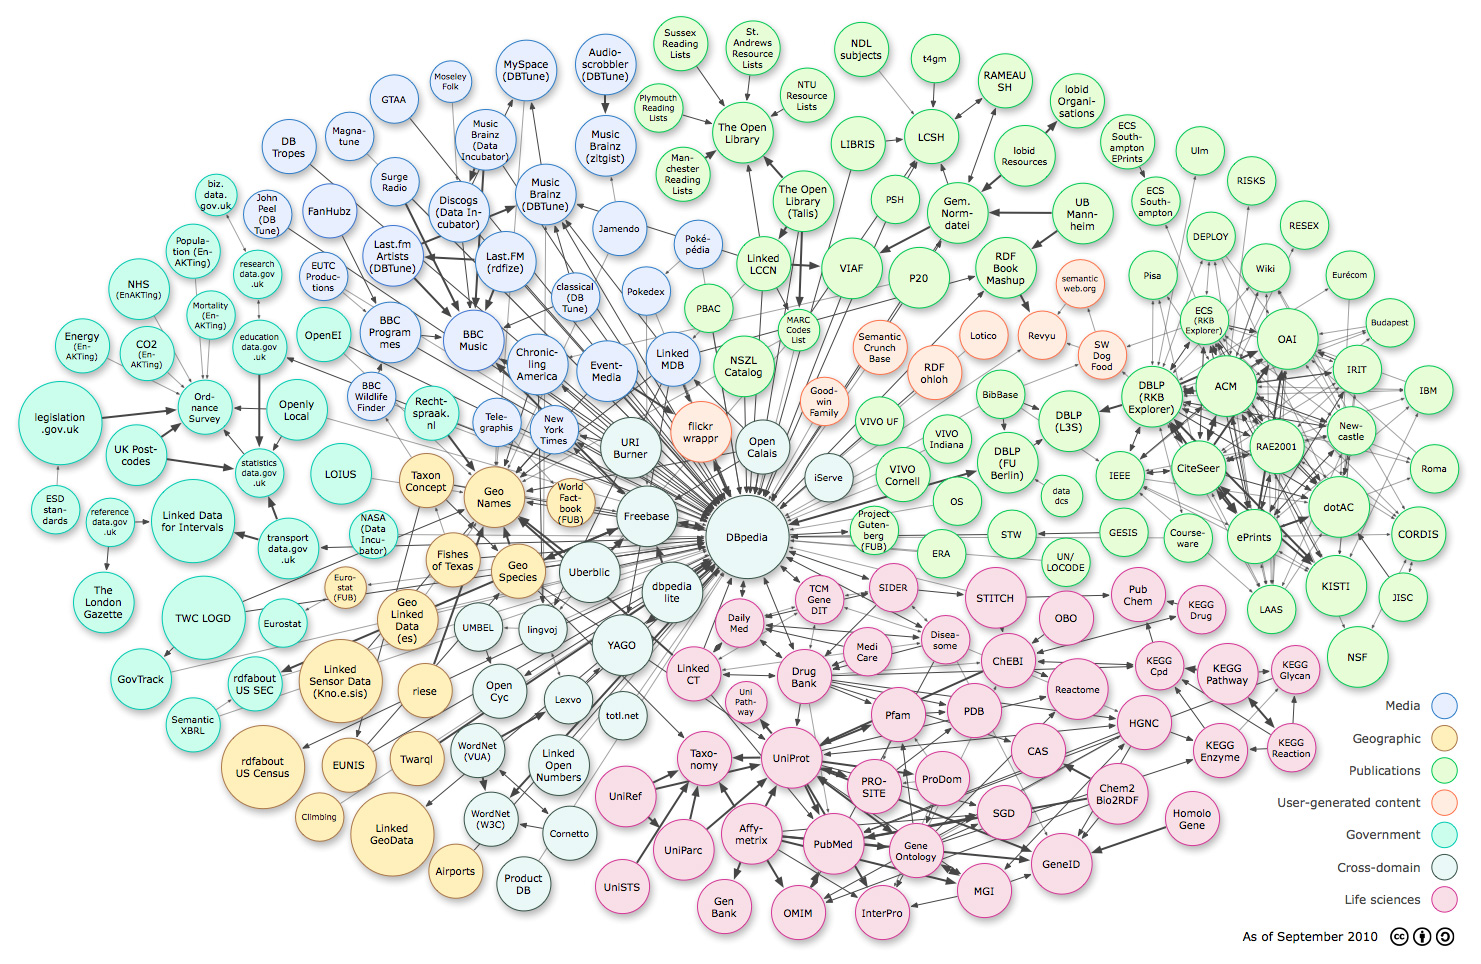
\includegraphics[width=\textwidth]{figures/opendata.jpeg}
\caption{Published open data}
\label{open data chart}
\end{figure}

For the first time we have been presented with a huge and interconnected data source with which anybody who has an internet connection can query freely. Nevertheless until today there have not emerged any killer application that can promote the concept of semantic web to a more broad audience. The usage of those data sources is rather limited for either academia or highly specialized application such as some bioinformatics query utilities.

Since semantic web is a more reasonable way to organize information, it should further facilitate information retrieval for our daily use. Tim Berners-Lee (2001) described an automatic personal agent that has the ability to retrieve data with the precision and recall as a human being. This agent is no near to be found until today, but using semantic linked data to optimize precision and recall of search result is an attainable goal.

Existing web search is keywords oriented. The search engine can skim through its indexed database for documents containing user provided keywords, or its synonyms. While according to Andrei Broder (2002), web queries can be categorized into three major classes: Informational, Navigational, and Transactional. Keyword search may not satisfy the different purposed queries with same or similar keywords.

Semantic search, on the other hand, may provide a better alternative because it integrated a more dynamic relationship structure of concepts, or ontologies.

Originally, ontology is a branch of philosophical study about the basic categories of being and their relations, which deals with questions concerning how entities can be grouped, related within a hierarchy, and subdivided according to similarities and differences.

It is intriguing that people begin to see this term more and more in the context of information system modelling rather than philosophy. Whether it is UML or Enhanced Entity Relationship Model, software engineers are pondering the inherent relationship between concepts in the focused domain.

The advent of semantic web made ontology even more relevant, as concepts in any data sources become openly accessible, so that different parties might impose different interpretations on those concepts, and its relationship with other concepts.

This becomes the purpose of the project, which is to show that the key feature of semantic web is that entities can be associated with a range of context. The prototype search engine will utilize semantic linked data to display different facets for the same topic. User could later browse to any particular facet by following the links between data entities.

Interestingly, this faceted approach of representing information is what our brains do during the cognitive process of thinking. When we need to refer to any particular thing, we generally speak of it in terms of the class to which it belongs. But we assign this classification upon the item being referred according to the problem we want to solve at hand. For example, under various circumstances, we might refer to Leonardo da Vinci as the artist, as the Italian or Tuscan painter, as the Renaissance artist, or even as the Italian vegetarian, or the person who was prosecuted under anti-homosexuality laws. When we refer to him by those classes, we are implying the relevant characteristics that Leonardo da Vinci had that share with other instances within the same class.

With available semantic linked data sources, we propose a novel semantic search approach to deliver a faceted information visualization upon a given fact, and a prototype software will be developed as a initial show case.

\section{Related Work}

Some existing applications, such as Google knowledge search or Facebook graph search, only work with data links on the instance level. That is to say they model the dataset as a graph. On a closer examination, both of them use a local data store instead of the whole data store network.

Facebook use an internal data store with API for external accessing. Google acquired Freebase as the basis for the knowledge search, which provides semantic search and RDF functionalities. It is built by importing various semantic data sources. But it does not maintain a well structured class hierarchy, or ontology, above its instance layer.

Till today, the class dimension of semantic linked data is largely untouched by applications. This is not caused by the lack of ontology information available on the internet. DBpedia, the semantic data store mirror for Wikipedia, maintained a shallow, cross-domain ontology. It has been manually created and currently covers 359 classes which form a subsumption hierarchy and are described by 1,775 different properties (Christopher Sahnwaldt, 2012). Some other well populated ontologies are YAGO and UMBEL (Upper Mapping and Binding Exchange Layer), both containing more than thousands of class definitions. Our prototype system will query all the above mentioned ontologies to enrich the query result.

\chapter{Task Performed}

\section{Feasibility study}

The most challenging part of designing a search engine is to answer the question that how the knowledge source is constructed and organized. Due to time and equipment limitations, for this prototype we will not build a local data store. In addition, it is necessary to use linked data published on the internet to ensure the most diverse coverage of facets of entities.

To realize this goal, we need a data source where the entities is covered by multiple ontologies. DBpedia is a semantic counter part of Wikipedia, and independently developed ontologies exist which describe the relations between entities in DBpedia with different specialized emphasis. After tested using its SPARQL endpoint to query the entity store and inter-source ontologies, we felt that DBpedia is stable, relatively fast, well maintained, and populated with sufficient amount of entities. So we chose DBpedia for our primary query destination.

SPARQL is a query language for RDF data stores. Currently there are more than 200 websites providing public SPARQL query functionality (as SPARQL endpoints). It specifies different query variations for different purposes. SELECT query returns the result in table format, and CONSTRUCT query returns the result in RDF graph format. SPARQL is used as our query language.

\section{Rapid prototyping}

We expect the end-user to provide keywords for the search. Keywords are not excellent to pinpoint one exact concept. Therefore the prototype will consist two major functionalities: Keywords disambiguation to let user determine one concept to be visualized, and concept visualization to display the relationship the chosen concept has with different classification schemas. 

\subsection{Disambiguation module}

We began with developing the disambiguation module first, starting as a command-line script with the first argument as input. We used a Python package SPARQLWrapper, which helps establish connections with a given SPARQL endpoint, send SPARQL query strings, and receive and convert the result to a specified format. Regular express module is used to build the query string so that the first letter of the given words will be case insensitive.

At the beginning we used a SELECT query. If an entity has attributes associated with multiple values, the result table will contain duplicate attributes names. Later we found out this will result in more code for book keeping during iterating through multiple valued attributes. Then we switch to CONSTRUCT query, where the query result is a RDF graph, that can be represented in XML or JSON format.

With this result, we imported the rdflib package for RDF manipulation. With a given RDF graph, it helps pick out the subject, predicate, or object if one of them is given as the confinement. Besides, it provides a wrapper class RDF resource, which can group all the RDF triple with the same URI together as an object, making message passing easier.

After querying DBpedia, topics sharing the user provided keywords in their titles are picked out from the result graph, wrapped as rdf resource, and packed in a list. The list is returned to the caller and displayed to the console. User then will tell the console which topic he or she is interested in further investigating.



\subsection{Visualization module}

After the user choose the topic, the RDF resource object of the topic will be passed to the visualization module. The networkx package will be invoked to store the topic and its ontology classifications as nodes. DBpedia triple store use the predicate "http://www.w3.org/1999/02/22-rdf-syntax-ns\#type" to denote the class-instance relationship. We will query the URI of the class, to further obtain information about:

\begin{center}
~\\
\end{center}
\begin{itemize}
\item Some other typical instances this class contains
\item Superclass/subclass of this class
\end{itemize}

The information will be used to construct the information graph around the user specified entity. There will be a directed link from instances to the class they belong to, and from subclasses to superclasses. For example in the graph the class of scientific fiction movie will be linked to the class movie.

Because in the topic resource object, we already have the class URIs as the objects in the triples with RDF:type predicate, so instead of using SPARQL for querying, we can directly obtain a RDF graph from the URI. Again rdflib has a parsing function to read in a RDF graph with the given URI, and later we wrap the graph into a rdflib resource object.

While querying the URI of the classes of the entity, we encountered another issue. Some ontology websites do not provide RDF triples with the URI link, but only a html formatted webpage. They might store the RDF formatted page at another place but for the moment we excluded querying those websites. We use regular expression to find URIs that contain "schema.org" or "opengis.net" for this reason.

At the early version of the visualization module we queried the URI of classes in a serial fashion. Several test runs revealed that if the connection to the URI was broken or lost, the parsing function of rdflib cannot terminate properly, and it does not have any time-out mechanism, which lead to the freeze of the program. One direct and probably only viable solution was to fork the URI parsing into a separate thread and use the main thread to time it out when needed. Consequently a subclass of Python's threading.Thread class was set up to realize the functionalities of querying and returning the result as either RDF graph or rdflib resource object.

Even with such configuration, querying class URIs was still taking a considerable amount of time, with an average of 2-3 seconds per URI and 6 class URIs per entity. This was especially unbearable after we moved the running environment from console to browser, where there was no real time feedback of what the script was doing. Afterwards we recognized that all the class URI querying can be perfectly parallelized, as we already had the thread class to spawn multiple threads. Now we use a Python built-in data structure Set to serve as the thread pool, and give all the threads 7 seconds for the parsing. The time limit is quite relax to ensure most of the fetching will success.

After the class related RDF is queried back, we can build the directed graph with the newly obtained triples to find relationships between classes, as well as some other typical instances that this class contains.

The networkx graph is returned to the caller. For the console version the output was firstly as a list of nodes and a list of links, and later we imported the package numpy and matplotlib for directed graph plotting. The limitation of styling provided by matplotlib and some other alternatives was one of the reasons we migrated the platform into browser based. For the browser to process the directed graph data, we dumped it into JSON format, which will be read by the JavaScript rendering functions.

\subsection{CGI server}

Some other reasons for us to choose a browser based application include simpler distribution and friendlier user experience. Python has several built-in packages for setting up http server, let alone third party support of running python script on various robust server applications. For the sake of demonstrating this prototype system, we chose one of the simplest form of the server, a Python built-in HTTPServer with a CGIHTTPRequestHandler. This request handler can run any script in the cgi-bin directory upon http request. Python also has a cgi module to pass http GET or POST parameters into the script.

To output HTML pages instead of printing results in the console, we refactored the code to make it more Model-View-Controller oriented. This lead us to use pickle for passing the list of rdflib resource objects between the two view generating scripts.

For the visualization of the graph data, which is stored in JSON format, we use a JavaScript library D3, which supports fully customizable graph representation. We developed a gravity enabled directed graph for better user interaction. Nodes are coloured differently for whether it is the original searched entity, the class to which it belongs, or other instances related to the classes. Labels of the nodes are designed to display their domain names for the purpose of demonstration, and can be adjusted for particular usage. Clicking the nodes will redirect the browser to the URI that the node bears.

For all the above mentioned tasks, we extensively referred to the documentations of Python, the Python packages used in this prototype system, and the D3 library. 

\chapter{Key points and tools}

\section{Git}

Using Git is like a breeze. Although as a first-timer, life without Git can hardly be remembered.

gitignore

ssh

\section{Python}

\subsection{SPARQLWrapper}

\subsection{rdflib}

\subsection{other packages}

\section{Regular expression}

\section{Multi-thread}

\chapter{How-to}

\chapter{Summary}
\section{Lesson learned}
\section{Future research}

property precedence

\chapter{Appendix}
\section{References}
\section{A brief summary of the papers}

%%\subsection{Footnotes}
%%The following command is used for footnotes \textbackslash footnote\{text for the footnote\}.\footnote{text for the footnote}

%%\subsection{URIs and eMail}
%%The \textbackslash url\{\} command is used to properly show an URI or e-mail address:

%%School of Graduate Studies: \url{www.mun.ca/sgs}\\
%%eMail: \url{eTheses@mun.ca}

%%------------List of Tables----------------------
%%\listoftables{}
%%\addcontentsline{toc}{chapter}{List of Tables}
%%------------List of Figures----------------------
%%\listoffigures{}
%%\addcontentsline{toc}{chapter}{List of Figures}

%ensure correct pagination for the bibliography in the table of contents
\cleardoublepage

 
\end{document}
